%!TEX TS-program = xelatex

\documentclass[a4paper,14pt]{article}

\usepackage{header}


\author{}
\title{}
\date{\today}

\begin{document} % конец преамбулы, начало документа
\section{Компонування поперечної рами будівлі}
\subsection{Компонування поперечної рами промислової будівлі}
\begin{enumerate}
\item Визначаємо висоту підкранової балки: при кроці 6 м:

$h_{\textit{п,б}}=1000$ мм

\item Визначити висоту над кранової $H_{\textit{в}}$ і підкранової $H_{\textit{н}}$ частин колони, повну висоту $H_{\textit{1}}$, $H$.

Вантажопідйомність $Q= 20\;{\textit{т}}$.

Висота $A=2400\;{\textit{мм}}$.

$H_{\textit{н}}=8600\;{\textit{мм}}$.

h кранового рельса =$70\;{\textit{мм}}$.

$H_{\textit{в}}=h_{\textit{п.б.}}+A+1000$=$1000+2400+100=3500\;\textit{мм}$.

$H_1=H_{\textit{н}}+H_{\textit{в}}=8000+3500=12100\;\textit{мм}$.

$H=H_1+150=12250\;\textit{мм}$.

Висота ферми при прольоті 18\;\textit{м}\;:

$H_{\textit{ф}}=2450\;\textit{мм}$.

\item Прив'язка $"a"$ розбивочної осі ряду колон:

-- нульова прив'язка.

\item Призначити висоту перетину над кранової частини колони $h_{\textit{верхнє}}$:

При нульовій прив'язці --- $380\;{\textit{мм}}$.

$h_{\textit{нижнє}}=\left(\dfrac{1}{10}\ldots\dfrac{1}{14}\right)H_\textit{н}=860\ldots614\;\textit{мм}$.

$b_{\textit{нижнє}},\;b_{\textit{верхнє}}=\left(\dfrac{1}{20}\ldots\dfrac{1}{25}\right)H_\textit{н}=430\ldots344\;\textit{мм}$.

Вид колони --- наскрізна.

Так як :$H_1<\textit{10,8}\;\textit{м}$; $h_\textit{нижнє}<\textit{900}\;\textit{м}$; $Q<\textit{30}\;\textit{т}$, проліт до 24 м, то приймаємо розміри колони:

$h_{\textit{гілки}}=200\;\textit{мм}$\;$h_{\textit{н}}=1000\;\textit{мм}$

$b_{\textit{нижнє}},\;b_{\textit{верхнє}}=400\;\textit{мм}$.
\end{enumerate}
\newpage
\begin{figure}[h]
    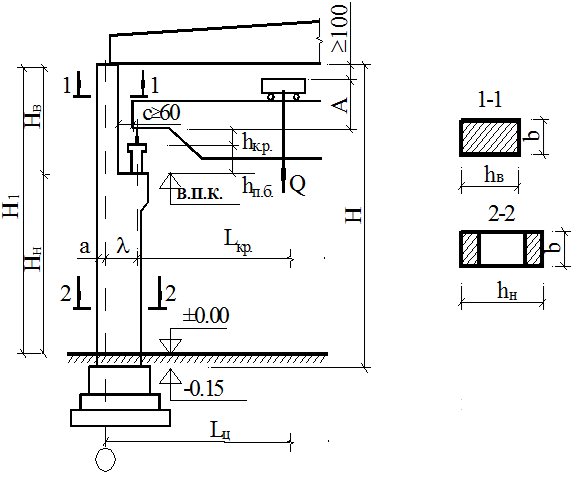
\includegraphics[width=\textwidth]{1_1.png}
    \caption{Схема поперечної рами.}\label{ris1_1} 
\end{figure}
%Сделать рисунок
\newpage
\section{Статичний розрахунок поперечної рами}

\textbf{Збір навантаження:}
\begin{figure}[h]
    \begin{center}
        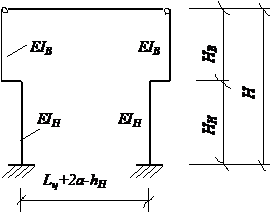
\includegraphics[scale=1]{2_1.png}
        \caption{Статична розрахункова схема рами промислових будівель.}\label{ris2_1} 
    \end{center}
\end{figure}

%Сделать таблицу
%Рис. 3.1.  Статична розрахункова схема рами промислових будівель:
%Рис. 3.2. Розрахункова схема кроквяної конструкції при визначенні опорної реакції RA
Розрахунковий проліт рами:

$l_0=L_{\textit{цеха}}-2с=17000-2\cdot 200=16600\;{\textit{мм}}$
\begin{figure}[h!]
    \begin{center}
        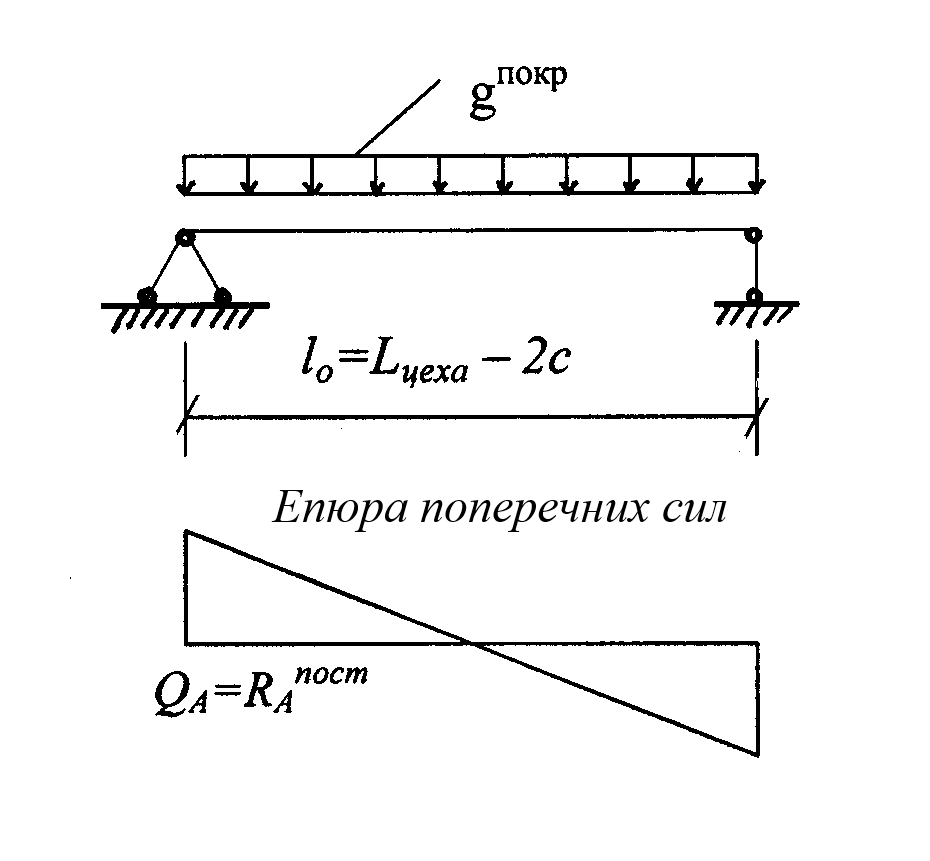
\includegraphics[scale=0.35]{2_22.png}
        \caption{Розрахункова схема кроквяної конструкції при визначенні
        опорної реакції $R_A$}\label{ris2_22} 
    \end{center}
\end{figure}

Визначення опорної реакції $R^{\textit{Пост}}_A$:

\begin{equation}
    R^{\textit{Пост}}_A=0,5\cdot g^{\textit{покр}}\cdot l_0 + {\textit{1,1}}\cdot {\textit{0,5}}\cdot G^{\textit{стр}}_{\textit{П}}
\end{equation}

де : $G^{\textit{стр}}_{\textit{П}}$ - маса кроквяної конструкції

$g^{\textit{покр}}$ - навантаження на покритті

 
\begin{equation}
    g^{\textit{покр}}=g_{\textit{р}}\cdot S_1
\end{equation}

де : $g_{\textit{р}}$ - розрахункове постійне навантаження на 1 м$м^{\textit{2}}$ плити покриття

$S_1$-крок поперечних рам в будівлі

$g^{\textit{покр}}={\textit{3,52}}\cdot 6 = {\textit{21,12}}\;\textit{кН/м}$

$R^{\textit{Пост}}_A=0,5\cdot {\textit{21,12}}\cdot {\textit{16,6}}+ {\textit{1,1}}\cdot {\textit{0,5}}\cdot 60={\textit{208,296}}\;{\textit{кН}}$

\textbf{Снігове навантаження}
\begin{figure}[h!]
    \begin{center}
        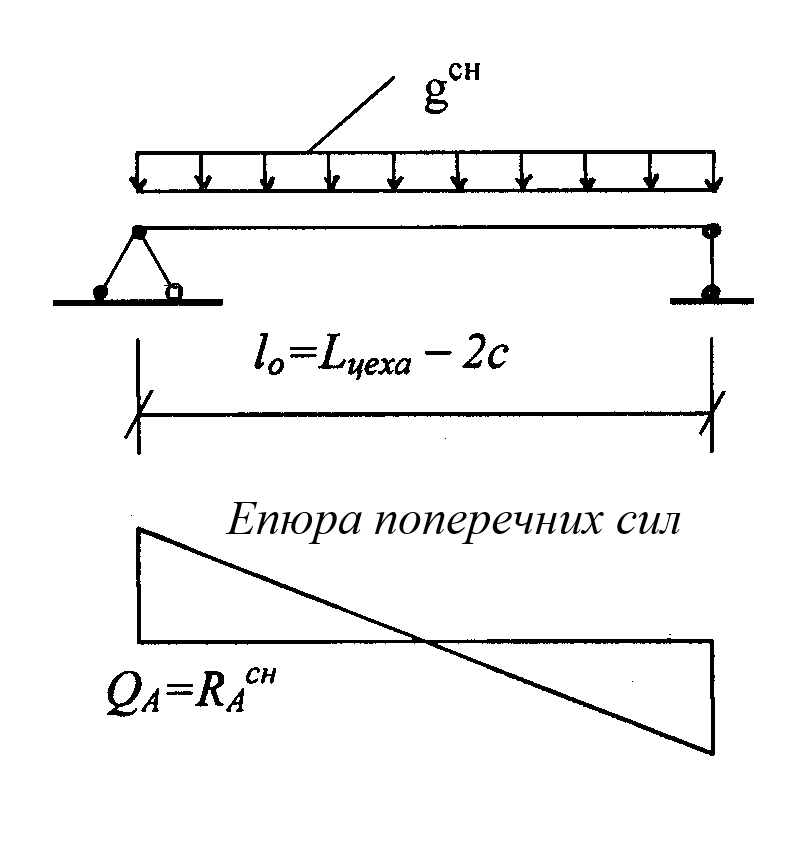
\includegraphics[scale=0.35]{2_222.png}
        \caption{Розрахункова схема кроквяної конструкції при визначенні
        опорної реакції $R_A$}\label{ris2_222} 
    \end{center}
\end{figure}
\begin{equation}
    p^{\textit{сн}}=S_{\textit{m}}\cdot S
\end{equation}
\begin{equation}
    S_m=\gamma_{fm}\cdot S_0 \cdot C
\end{equation}

де : $\gamma_{fm}$- коеф. надійності для середн. періоду повтрюваності снігового навантаження Т = 60 років 

$S_0$ - характеристичне значення снігового навантаження на 1 м$м^{\textit{2}}$ для заданого району будівництва

C = 1 при відсутності даних про режим експлуатації будівлі с плоскою конструкцією покрівлі і розміщенням його на висоті H < ${\textit{0,5}}$ км над рівнем моря.

$S_m=1,04\cdot 1400\cdot 1=1456\;\textit{Па}=1,456\;{\textit{кН/м}}^2$

$p^{\textit{сн}}=1,456\cdot 6=8,736\;\textit{кН/м}$

\begin{equation}
    R^{\textit{cн}}_A=0,5\cdot p^{\textit{сн}}\cdot l_0
\end{equation}

$R^{\textit{cн}}_A=0,5\cdot 8,736 \cdot 16,6 = 72,51\;\textit{кН/м}$

\textbf{Кранове навантаження}
\begin{figure}[h]
    \begin{center}
        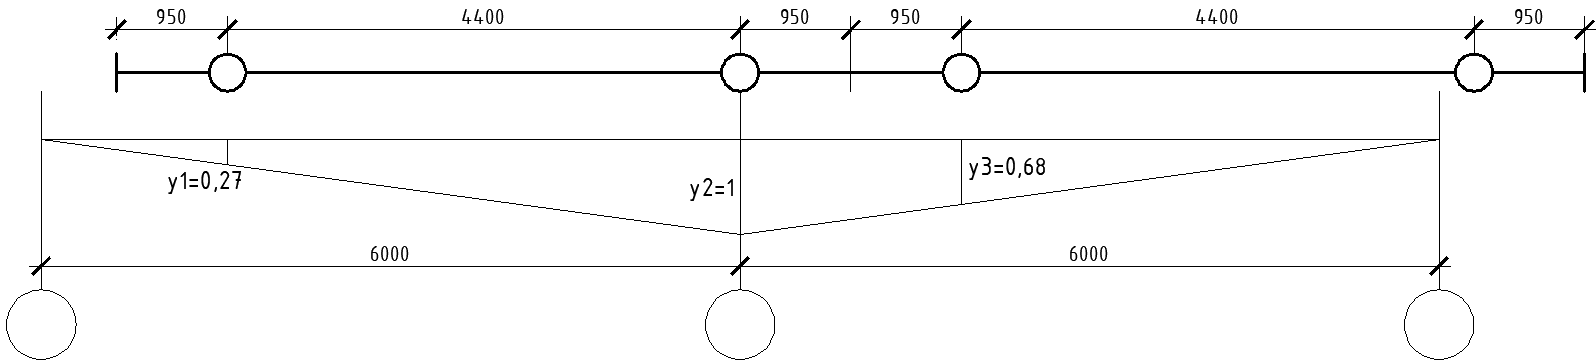
\includegraphics[width=\textwidth]{2_3.png}
        \caption{Схема розташування двох зближених мостових кранів на
        підкрановій балці для визначення кранових навантажень на поперечну раму
        будівлі.}\label{ris2_3} 
    \end{center}
\end{figure}

Проліт крана $L_k$=$\textit{16,6}\;\textit{м}$

Ширина крана $B=6300\;\textit{мм}$

База крана $K=4400\;\textit{мм}$

$H=2400\;\textit{мм}$

$B_1=260\;\textit{мм}$

$P^n_{max}$-навантаження коліс на підкранові рейки-$195\;\textit{кН}$

Вага візка - $8,5\;\textit{т}$

G - Вага крана з візком -$28,5\;\textit{т}$

Тип кранової рейки - КР70

%вставить рисунок линий влияния


\begin{equation}
    D_{max}=\gamma_{fm}\cdot \psi \cdot P^n_{max} \cdot \sum y_i
\end{equation}

де: $\gamma_{fm}$ - см. п. 7.9 %[]

$\psi$ - см. п. 7.22 %[]

$\sum y_i$ - Рис. \ref{ris2_3}.

\begin{equation}
    D_{min}=\gamma_{fm}\cdot \psi \cdot P^n_{min} \cdot \sum y_i
\end{equation}

\begin{equation}
P^n_{min} = \dfrac {Q+G}{n_0}-P^n_{max}
\end{equation}

де : $n_o$ - кількість коліс на одній стороні крана

$D_{max}=1,1\cdot 0,85 \cdot 195 \cdot 1,95$ = $355,534\;\textit{кН}$

$P^n_{min} = \dfrac {200+285}{2}-195$=$47,5\;\textit{кН}$

$D_{min}=1,1\cdot 0,85 \cdot 47,5 \cdot 1,95$ = $86,6\;\textit{кН}$

Навантаження на раму від поперечного гальмування

\begin{equation}
    T=\gamma_\textit{соч}\cdot \gamma_f \cdot T^\textit{кол}_{n} \cdot \sum y_i
\end{equation}

Горизонтальне поперечне гальмівне навантаження від одного колеса 
   для кранів з гнучким підвісом вантажу 

\begin{equation}
    T^\textit{кол}_{n}=\dfrac {0,05\cdot (Q+Q_t)}{n_0}
\end{equation}

$T^\textit{кол}_{n}=\dfrac {0,05\cdot (20+8,5)}{2}=\textit{0,7125}\;\textit{т}=\textit{7,2}\;\textit{кН}$

$T=0,85\cdot 1,2 \cdot 7,2 \cdot 1,95 = \textit{14,32}\;\textit{кН}$

Навантаження від стінових панелей:

\begin{equation}
    G_\textit{стпн}= S \cdot Н_\textit{н}\cdot g
\end{equation}

$G_\textit{стпн}= 6 \cdot 8,6\cdot 2,8 = 144,48\;\textit{кНм}$

\begin{equation}
    G_\textit{стпн.в.}= S \cdot Н_\textit{в}\cdot g
\end{equation}

$G_\textit{стпн.в.}= 6 \cdot 3,5\cdot 2,8= 58,8\;\textit{кНм}$

Вітрове навантаження

Граничне розрахункове значення вітрового навантаження:

\begin{equation}
    W_\textit{m}= \gamma_{fm} \cdot W_\textit{0}\cdot C
\end{equation}

де:  $\gamma_{fm}$ ---  коефіцієнт надійності, в залежності від терміну повторності максимального значення вітрового тиску в роках. На 100 років --- $\gamma_{fm}$ = 1,14

$W_\textit{0}$ --- характеристичне значення вітрового тиску, залежне від району будівництва. $W_\textit{0} - 0,47\;\textit{кНм}^2$

$h=5\;\textit{м} = W_{5}= 0,47\cdot 0,4 = 0,188\;\textit{кНм}^2$

$h=10\;\textit{м} = W_{10}= 0,47\cdot 0,6 = 0,282\;\textit{кНм}^2$

$h=20\;\textit{м} = W_{20}= 0,47\cdot 0,85 = 0,399\;\textit{кНм}^2$

Еквівалентне вітрове навантаження $W_e$

\begin{equation}
    W_\textit{e}= \dfrac{2M_3}{H^2}
\end{equation}

$M_3 = \dfrac{0,188\cdot 12,25^2}{2}+\dfrac {1}{2}\cdot (0,308-0,188)\cdot 7,25 \cdot \left(\dfrac {2}{3}\cdot 7,25 + 5\right)= 18,4\;\textit{кНм}^2$ 

$W_\textit{e}= \dfrac{2\cdot 18,4}{12,25^2}= 0,245\;\textit{кНм}^2$ 

Активний вітер 

\begin{equation}
    W_\textit{a}= W_\textit{e} \cdot B\cdot C_{aer}\cdot \gamma_{fm} 
\end{equation}

$W_\textit{a}= 0,245 \cdot 6\cdot 0,8\cdot 1,14 = 1,341\;\textit{кН/м.п.}$   

Пасивний вітер

$W_\textit{п}= 0,245 \cdot 6\cdot 0,6\cdot 1,14 = 1,01\;\textit{кН/м.п.}$ 

Зосереджена сила на рівні верха колон по середньому вітряному тиску між $0,308\;\textit{кНм}^2$ і $0,337\;\textit{кНм}^2$

$W = \left(\dfrac{0,308+0,337}{2}\right)\cdot 6 \cdot 2,45 \cdot (0,8+0,6)\cdot 1,14 = 7,57\;\textit{кН}$ 

%Вставить рисунок разреза ветра

Статична розрахунок поперечної рами 

%<<<<<<< HEAD
\begin{enumerate}
    \item Момент інерції відносно осі Y:
    \begin{equation}
        I_z = \dfrac{b\cdot h^3_\textit{в}}{12}+\dfrac{bh-(H_\textit{н}-h_\textit{в})^2}{2} 
    \end{equation}
    
    $$I_z = \dfrac{40\cdot 20^3}{12}+\dfrac{40\cdot 20-(100-20)^2}{2}=23866,66\;\textit{см}^4$$

    $EF=3310000\cdot (0,4\cdot 0,2) = 264800\;\textit{т}$

    $I_y = 40 \cdot 20\cdot 40^2 = 0,0064\;\textit{см}^2$

    $EI_y = 3310000\cdot 0,064 = 21184$
%Вставить рисунок с сечением колон

    \item Розрахункове поєднання зусиль
    
    \textbf{Елемент 1, переріз 1}
    \begin{equation*}
        \begin{aligned}
        1+2&+3+4-7\qquad  &1+&3+6+7 &1+2&+3+4-7\\
        M^+_y &= \textbf{+265,99} &M^-_y &= \textbf{-193,405}\qquad &N^-_{max} &= -719,658\\
        N_\textit{відп} &= -719,658  &N_\textit{відп} &= -597,47 &M_\textit{відп} &= +265,99 \\
        Q_\textit{z.відп} &= -41,052 &Q_\textit{z.відп} &= 18,078 &Q_\textit{z.відп} &= -41,052 \\
        \dfrac{M}{N}&=0,369  &\dfrac{M}{N}&=0,323 &\dfrac{M}{N}&=0,369 
        \end{aligned}
    \end{equation*}
 
    \textbf{Елемент 1, переріз 2}
    \begin{equation*}
        \begin{aligned}
        1+2&+3+6-8\qquad  &1+&2+3+4\\
        M^-_y &= -103,237 &N^-_{max} &= -682,55 \\
        N_\textit{відп} &= -629,63  &M_\textit{відп} &= -39,418\\
        Q_\textit{z.відп} &= 3,701 &Q_\textit{z.відп} &= 22,14 \\
        \dfrac{M}{N}&=0,16  &\dfrac{M}{N}&=0,05  
        \end{aligned}
    \end{equation*}
        \textbf{Елемент 3, переріз 1}
        \begin{equation*}
        \begin{aligned}
        1&+2+4  &1&+6 &1&+2\\
        M^+_y &= \textbf{+72,771} &M^- &= -3,62 &N^-_{max} &= -316,008\\
        N_\textit{відп} &= -308,311\qquad  &N_\textit{відп} &= -239044\qquad &M_\textit{відп} &= +39,742 \\
        Q_\textit{z.відп} &= -22,14 &Q_\textit{z.відп} &= 2,835 &Q_\textit{zвідп} &= -10,888 \\
        \dfrac{M}{N}&=0,23  &\dfrac{M}{N}&=0,01 &\dfrac{M}{N}&=0,12
        \end{aligned}
        \end{equation*}
        \textbf{Елемент 3, переріз 2}
        \begin{equation*}
        \begin{aligned}
        &1+2  &1&+2+4\\
        N^-_{max} &= -301,046\qquad &Q_z &= -10,888 \\
        Q^-_\textit{z.відп} &= 17,735 &N^-_\textit{відп} &= -293,349 \\
        \end{aligned}
        \end{equation*}

        Від постійного навантаження

        \textbf{Елемент 1, переріз 1}
        \begin{equation*}
            \begin{aligned}
            &\quad1  \\
            N &= 277,49 \\
            M_y &= 26,653  \\
            Q &= -8,242 \\
            \end{aligned}
            \end{equation*}
        \textbf{Елемент 1, переріз 2}
        \begin{equation*}
            \begin{aligned}
            &\quad1  \\
            N &= -240,381 \\
            M_y &= -44,228  \\
            Q &= -8,242 \\
            \end{aligned}
            \end{equation*}
        \textbf{Елемент 3, переріз 1}
        \begin{equation*}
            \begin{aligned}
            &\quad1  \\
            N &= -239,044 \\
            M_y &= 30,083  \\
            Q &= -8,242 \\
            \end{aligned}
            \end{equation*}
            \textbf{Елемент 3, переріз 2}
        \begin{equation*}
            \begin{aligned}
            &\quad1  \\
            N &= -277,049 \\
            M_y &= -26,65+3  \\
            Q &= -8,242 \\
            \end{aligned}
            \end{equation*}
\end{enumerate}
%=======

%>>>>>>> c66bf3aeb27969b09cea77f323300f71c1fbe802


\newpage
\section{Проектування колони одноповерхової промислової будівлі}
\subsection{Розрахунок поздовжньої арматури колони}

\begin{enumerate}
    \item Обчислюємо ексцентриситет:
        \begin{equation}\label{eq:e_0}
            e_0 = \dfrac{M}{N}+e_a
        \end{equation}
        де: \begin{itemize}
                \item $e_a = \dfrac{1}{600} \cdot 8600 = 14,3\;\textit{мм}$
                \item $e_a = \dfrac{1}{30} \cdot 200 = 6,6\;\textit{мм}$
            \end{itemize}
        Обираємо $e_a = 14,3\;\textit{мм}$
        $$e_0 = \dfrac{265,99}{219,688}+0,014 = 0,384\;\textit{м}$$
    \item Наведений радіус інерції перерізу підкранової частини двогілкової колони:
        \begin{equation}
            i_{red}^2 = \dfrac{c^2}{4 \left(\dfrac{1+3c^2}{\psi^2n^2h^2}\right)}
        \end{equation}
        де: $\psi^2 = 1,5$

                $n = \dfrac{H_\textit{н}}{S} = \dfrac{8,6}{2} = 4,3\;\textit{м}$

                $S = (8 \ldots 10)h = 10 \cdot 0,2 = 2\;\textit{м}$
           
        $$i_{red}^2 = \dfrac{0,8^2}{4 \left(\dfrac{1+3 \cdot 0,8^2}{1,5 \cdot 4,3^2 \cdot 0,2^2}\right)} = 0,05859\;\textit{м}$$
    \item Приведена гнучкість підкранової частини колони:
        \begin{equation}
            \lambda_{red} = \dfrac{l_0}{i_{red}^2}
        \end{equation}
        де: $l_0 = 1,5H_\textit{н} = 1,5 \cdot 8,6 = 12,9\;\textit{м}$
        $$\lambda_{red} = \dfrac{12,9}{0,05859} = 220,17$$
        
        Гранична гнучкість:
        \begin{equation}
            \lambda \lim = \dfrac{20ABC}{\sqrt{n}}
        \end{equation}
        де: $n = \dfrac{N}{A_cf_{cd}} = \dfrac{719,658 \cdot 10^3}{2(0,4 \cdot 0,2) \cdot 17 \cdot 10^6} = 0,265$

            $A = \dfrac{1}{(1+0,2\phi_{ef})} = \dfrac{1}{(1+0,2 \cdot 2)} = 0,71$

            $\phi_{ef} = 2$

            $B = 1,1$

            $C = 0,7$
            $$\lambda\lim = \dfrac{20 \cdot 0,71 \cdot 1,1 \cdot 0,7}{\sqrt{0,265}} = 21,61$$

        Так як, $\lambda_{red} > \lambda\lim$ слід враховувати вплив прогину на величину ексцентриситету повздовжньої сили. В цьому випадку в розрахунку замість $e_0$ необхідно використовувати
        величину $(\eta \cdot l_0)$, де 
        \begin{equation}
            \eta = \dfrac{1}{1 - \dfrac{N}{N_{cr}}}
        \end{equation}
        \begin{equation}
            N_{cr} = \dfrac{6,4E_{cm}}{l_0^2}\left[\dfrac{I}{\phi_l}\left(\dfrac{0,11}{0,1 + \dfrac{\sigma_e}{\phi_p}} + 0,1\right) + \alpha I_s\right]
        \end{equation}
        $I = 2\left[\dfrac{bh^3}{12} + bh \left(\dfrac{c}{2}\right)^2\right] = 2\left[\dfrac{0,4 \cdot 0,2^3}{12} + 0,4 \cdot 0,2 \left(\dfrac{0,8}{2}\right)^2\right] = 0,02613\;\textit{м}^4$

        $\phi_l = 1 + \beta \dfrac{M_1}{M} = 1 + 1 \cdot \dfrac{26,653}{265,99} = 1,1 < (1 + \beta)$

        $I_S = 2 \rho bh \left(\dfrac{c}{2}\right)^2 = 2 \cdot 0,02 \cdot 0,4 \cdot 0,2 \cdot \left(\dfrac{0,8}{2}\right)^2 = 0,000512\;\textit{м}^4$

        $\sigma_e = \dfrac{l_0}{h_\textit{н}} = \dfrac{12,9}{1} = 12,9\;\textit{м}$

        $\phi_p = 1$

        $\alpha = \dfrac{E_S}{E_{ct}} = \dfrac{210\;\textit{Па}}{32,5\;\textit{Па}} = 6,46$
        $$N_{cr} = \dfrac{6,4 \cdot 32500 \cdot 10^6}{12,9^2} \left[\dfrac{0,02613}{1,1} \left(\dfrac{0,11}{0,1 + \dfrac{12,9}{1}} + 0,1\right) + 6,46 \cdot 0,000512\right]$$
        $$N_{cr} = 7354530\;\textit{Па} = 7354,53\;\textit{кН}/\textit{м}^2$$
        $$\eta = \dfrac{1}{1 - \dfrac{719,658}{7354,53}} = 1,11$$
    \item Визначаємо зусилля в гілках колони:
        \begin{equation}
            N_{\textit{в}1,2} = 0,5N \pm \dfrac{M \cdot \eta}{c}
        \end{equation}
        $$N_{\textit{в}1,2} = 0,5\cdot 719,658 + \dfrac{265,99 \cdot 1,1}{0,8} = 713,2\;\textit{кН}$$
        \begin{equation}
            M_\textit{в} = V \dfrac{S}{4}
        \end{equation}
        $$M_\textit{в} = 41,052 \cdot \dfrac{2}{4} = 20,526\;\textit{кН}$$
    \item Для кожної з гілок визначаємо:
        \begin{equation}
            e_0 = \dfrac{M_\textit{в}}{N_\textit{в}} + l_a
        \end{equation}
        \begin{equation}
            e = e_0\eta +  0,5h - a
        \end{equation}
        $\eta = 1$

        $h = 200\;\textit{мм}$

        $a = 30\;\textit{мм}$

        $d = h - a = 200 - 30 = 170\;\textit{мм}$

        $l_a = 200 / 30 = 6,6\;\textit{мм}$

        $\dfrac{S}{600} = \dfrac{2000}{600} = 3,33\;\textit{мм}$
        $$e_0 = \dfrac{20,526}{713,2} + 0,0066 = 0,035\;\textit{м}$$
        $$e = 0,035 \cdot 1 +  0,5 \cdot 0,2 - 0,03 = 0,105\;\textit{м}$$
    \item Підбираємо армування при несиметричному армуванні:
        \begin{equation}
            A_S^\prime = \dfrac{N \cdot e - 0,4 \cdot f_{cd} \cdot b \cdot d^2}{f_{yd} \cdot (d - a^\prime)} \geqslant 0
        \end{equation}
        $$A_S^\prime = \dfrac{713,2 \cdot 10^3 \cdot 0,105 - 0,4 \cdot 17 \cdot 10^6 \cdot 0,4 \cdot 0,17^2}{365 \cdot 10^6 \cdot (0,17 - 0,03)} \geqslant 0$$
        $$A_S^\prime = -0,0000728376\;\textit{м}^2$$

        Висновок --- переріз арматури приймаємо конструктивно.
        \begin{equation}
            A_S = \dfrac{0,55 \cdot f_{cd} \cdot b \cdot d - N}{f_{yd}} + A_S^\prime
        \end{equation}
        $$A_S = \dfrac{0,55 \cdot 17 \cdot 10^6 \cdot 0,4 \cdot 0,17 - 713,2 \cdot 10^3}{365 \cdot 10^6} +(-0,0000728376)$$
        $$A_S = -0,000284892\;\textit{м}^2$$

        Висновок --- переріз арматури приймаємо конструктивно.

        Підбираємо арматуру за відсотком армування:

        $A_S^\prime$ приймаємо $4\varnothing12A400C$ --- $A = 4,52\;\textit{см}^2$

        $A_S$ приймаємо $4\varnothing12A400C$ --- $A = 4,52\;\textit{см}^2$
        \begin{equation}
            \rho = \dfrac{A_S^\prime + A_S}{b \cdot d} \cdot 100\%
        \end{equation}
        $$\rho = \dfrac{4,52 + 4,52}{40 \cdot 20} \cdot 100\% = 1,13\%$$
        Оптимальне значення армування для колон 1\ldots 3\%    
\end{enumerate}
%Добавить ссылки на формулы
\textbf{Розрахунок за другою комбінацією зусиль.}
\begin{enumerate}
    \item Обчислюємо ексцентриситет за формулою (\ref{eq:e_0}):
        
        де: \begin{itemize}
                \item $e_a = \dfrac{1}{600} \cdot 8600 = 14,3\;\textit{мм}$
                \item $e_a = \dfrac{1}{30} \cdot 200 = 6,6\;\textit{мм}$
            \end{itemize}
        Обираємо $e_a = 14,3\;\textit{мм}$
        $$e_0 = \dfrac{193,405}{597,47}+0,014 = 0,34\;\textit{м}$$
    \item Наведений радіус інерції перерізу підкранової частини двогілкової колони (link):  
        $$i_{red}^2 = \dfrac{0,8^2}{4 \left(\dfrac{1+3 \cdot 0,8^2}{1,5 \cdot 4,3^2 \cdot 0,2^2} \right)} = 0,05859\;\textit{м}$$
    \item Приведена гнучкість підкранової частини колони (link):
        $$\lambda_{red} = \dfrac{12,9}{0,05859} = 220,17$$
        
        Гранична гнучкість (link):

        де: $n = \dfrac{N}{A_cf_{cd}} = \dfrac{597,47 \cdot 10^3}{2(0,4 \cdot 0,2) \cdot 17 \cdot 10^6} = 0,22$

            $A = \dfrac{1}{(1+0,2\phi_{ef})} = \dfrac{1}{(1+0,2 \cdot 2)} = 0,71$

            $\phi_{ef} = 2$

            $B = 1,1$

            $C = 0,7$
            $$\lambda\lim = \dfrac{20 \cdot 0,71 \cdot 1,1 \cdot 0,7}{\sqrt{0,22}} = 23,31$$

        Так як, $\lambda_{red} > \lambda\lim$ слід враховувати вплив прогину на величину ексцентриситету повздовжньої сили. В цьому випадку в розрахунку замість $e_0$ необхідно використовувати
        величину $(\eta \cdot l_0)$ за формулами (link) (link)
        
        $I = 0,02613\;\textit{м}^4$

        $\phi_l = 1 + 1 \cdot \dfrac{44,228}{193,405} = 1,23 < (1 + \beta)$

        $I_S = 0,000512\;\textit{м}^4$

        $\sigma_e = 12,9\;\textit{м}$

        $\phi_p = 1$

        $\alpha = 6,46$
        $$N_{cr} = \dfrac{6,4 \cdot 32500 \cdot 10^6}{12,9^2}\left[\dfrac{0,02613}{1,23}\left(\dfrac{0,11}{0,1 + \dfrac{12,9}{1}} + 0,1\right) + 6,46 \cdot 0,000512\right]$$
        $$N_{cr} = 7014160\;\textit{Па} = 7014,16\;\textit{кН}/\textit{м}^2$$
        $$\eta = \dfrac{1}{1 - \dfrac{597,47}{7014,16}} = 1,1$$
    \item Визначаємо зусилля в гілках колони за формулами (link), (link):
        $$N_{\textit{в}1,2} = 0,5 \cdot 597,47 - \dfrac{193,405 \cdot 1,1}{0,8} = 32,803\;\textit{кН}$$
        $$M_\textit{в} = 18,078 \cdot \dfrac{2}{4} = 9,039\;\textit{кН}$$
    \item Для кожної з гілок за формулами (link), (link) визначаємо:

        $\eta = 1$

        $h = 200\;\textit{мм}$

        $a = 30\;\textit{мм}$

        $d = 170\;\textit{мм}$

        $l_a = 6,6\;\textit{мм}$

        $\dfrac{S}{600} = 3,33\;\textit{мм}$
        $$e_0 = \dfrac{9,039}{32,803} + 0,0066 = 0,28\;\textit{м}$$
        $$e = 0,28 \cdot 1 +  0,5 \cdot 0,2 - 0,03 = 0,35\;\textit{м}$$
    \item Підбираємо армування при несиметричному армуванні за формулами\\(link),(link):
        $$A_S^\prime = \dfrac{32,803 \cdot 10^3 \cdot 0,35 - 0,4 \cdot 17 \cdot 10^6 \cdot 0,4 \cdot 0,17^2}{365 \cdot 10^6 \cdot (0,17 - 0,03)} \geqslant 0$$
        $$A_S^\prime = -0,00131364\;\textit{м}^2$$

        Висновок --- переріз арматури приймаємо конструктивно.
        $$A_S = \dfrac{0,55 \cdot 17 \cdot 10^6 \cdot 0,4 \cdot 0,17 - 32,803 \cdot 10^3}{365 \cdot 10^6} +(-0,00131364)$$
        $$A_S = 0,000338407,\;\textit{м}^2$$

        Висновок --- переріз арматури приймаємо конструктивно.

        Підбираємо арматуру за відсотком армування (link):

        $A_S^\prime$ приймаємо $4\varnothing12A400C$ --- $A = 4,52\;\textit{см}^2$

        $A_S$ приймаємо $4\varnothing12A400C$ --- $A = 4,52\;\textit{см}^2$
        $$\rho = \dfrac{4,52 + 4,52}{40 \cdot 20} \cdot 100\% = 1,13\%$$
        Оптимальне значення армування для колон 1\ldots 3\%
\end{enumerate}
\textbf{Розрахунок надкранової частини колони} %Сделать эскиз
\begin{enumerate}
    \item Обчислюємо ексцентриситет за формулою (\ref{eq:e_0}),
    де: \begin{itemize}
            \item $e_a = \dfrac{1}{600} \cdot H_\textit{в} =\dfrac{1}{600} \cdot 3500 = 5,83\;\textit{мм}$
            \item $e_a = \dfrac{1}{30} \cdot 380 = 12,6\;\textit{мм}$
        \end{itemize}
    Обираємо $e_a = 12,6\;\textit{мм}$
    $$e_0 = \dfrac{72,771}{308,311}+0,0126 = 0,25\;\textit{м}$$
\item Наведений радіус інерції перерізу підкранової частини двогілкової колони:
    \begin{equation}
        i_{red} = 0,289 \cdot h
    \end{equation}
    $$ i_{red} = 0,289 \cdot 0,38 = 0,11\;\textit{м}$$
\item Приведена гнучкість підкранової частини колони за формулою (link):
    
    де: $l_0 = 2H_\textit{в} = 2 \cdot 3,5 = 7\;\textit{м}$
    $$\lambda_{red} = \dfrac{7}{0,11} = 63,63$$
    Гранична гнучкість за формулою (link):
    
    де: $n = \dfrac{N}{A_cf_{cd}} = \dfrac{308,311 \cdot 10^3}{0,4 \cdot 0,38 \cdot 17 \cdot 10^6} = 0,12$

        $A = \dfrac{1}{(1+0,2\phi_{ef})} = \dfrac{1}{(1+0,2 \cdot 2)} = 0,71$

        $\phi_{ef} = 2$

        $B = 1,1$

        $C = 0,7$
        $$\lambda\lim = \dfrac{20 \cdot 0,71 \cdot 1,1 \cdot 0,7}{\sqrt{0,12}} = 31,56$$

    Так як, $\lambda_{red} > \lambda\lim$ слід враховувати вплив прогину на величину ексцентриситету повздовжньої сили. В цьому випадку в розрахунку замість $e_0$ необхідно використовувати
    величину $(\eta \cdot l_0)$ за формулами (link) (link), де: 
    
    $I = \dfrac{b \cdot h^3}{12} = \dfrac{0,4 \cdot 0,38^3}{12} = 0,0126\;\textit{м}^4$

    $\phi_l = 1 + \beta \dfrac{M_1}{M} = 1 + 1 \cdot \dfrac{30,083}{72,771} = 1,41 < (1 + \beta)$

    $I_S = \rho \cdot \left(\dfrac{d - a}{h}\right)^2 = 0,02 \cdot \left(\dfrac{0,35 - 0,03}{0,38}\right)^2 = 0,0142\;\textit{м}^4$

    $\sigma_e = \dfrac{l_0}{h_\textit{н}} = \dfrac{7}{0,38} = 18,42\;\textit{м}$

    $\sigma_{min} = 0,5 - 0,01 \cdot \dfrac{\sigma_e}{h} - 0,01f_{cd} =  0,5 - 0,01 \cdot \dfrac{18,42}{0,38} - 0,01 \cdot 17 = -0,155$

    $\phi_p = 1$

    $\alpha = \dfrac{E_S}{E_{ct}} = \dfrac{210\;\textit{Па}}{32,5\;\textit{Па}} = 6,46$
    $$N_{cr} = \dfrac{6,4 \cdot 32500 \cdot 10^6}{7^2}\left[\dfrac{0,0126}{1,41}\left(\dfrac{0,11}{0,1 + \dfrac{18,42}{1}} + 0,1\right) + 6,46 \cdot 0,0142\right]$$
    $$N_{cr} = 393412000\;\textit{Па} = 393412\;\textit{кН}/\textit{м}^2$$
    $$\eta = \dfrac{1}{1 - \dfrac{308,311}{393412}} = 1$$
  
\item Підбираємо армування при симетричному армуванні:
    \begin{equation}
        A_S = A_S^\prime = \dfrac{N \cdot e_0 - f_{cd} \cdot b \cdot h \cdot (d - 0,5h)}{f_{yd} \cdot (d - a^\prime)} \geqslant 0
    \end{equation}
    $$A_S = A_S^\prime = \dfrac{308,311 \cdot 10^3 \cdot 0,25 - 17 \cdot 10^6 \cdot 0,4 \cdot 0,38 \cdot (0,35 - 0,5 \cdot 0,38)}{365 \cdot 10^6 \cdot (0,35 - 0,03)}$$
    $$A_S = A_S^\prime = -0,0028\;\textit{м}^2$$

    Висновок --- переріз арматури приймаємо конструктивно.

    $A_S = A_S^\prime$ приймаємо $4\varnothing12A400C$ --- $A = 4,52\;\textit{см}^2$
\end{enumerate}
\subsection{Розрахунок розпірки двогілкової колони}
    \begin{enumerate}
        \item Згинальний момент в розпірці
        \begin{equation}
            M_{ds} = \pm \dfrac{V \cdot s}{2} 
        \end{equation}
        $$M_{ds} = - \dfrac{41,052 \cdot 2}{2} = -41,052\;\textit{кНм}$$
        \item Необхідна площа поздовжньої арматури при симетричному армуванні без врахування роботи бетону
        \begin{equation}
            A_S = A_S^\prime = \dfrac{M_{ds}}{f_{yd} \cdot (d - a^\prime)}
        \end{equation} 
        $$A_S = A_S^\prime = - \dfrac{41,052 \cdot 10^3}{365 \cdot 10^6 \cdot (0,36 - 0,04)} = -0,0003514\;\textit{м}^2$$
        $A_S = A_S^\prime$ приймаємо $3\varnothing14A400C$ --- $A = 4,61\;\textit{см}^2$
        \item Поперечна сила в розпірці
        \begin{equation}
            V_{ds} = \dfrac{2M_{ds}}{c} = \dfrac{V \cdot s}{c}
        \end{equation}
        $$V_{ds} = \dfrac{41,052 \cdot 2}{0,8} = 102,63\;\textit{кН}$$
        \item Умова необхідності розрахунку поперечних стрижнів розпірки
        \begin{equation}
            V_{Rd,c} = \left[C_{Rd,c} \cdot k \cdot \left(100 \cdot \rho_1 \cdot f_{ck,prism}\right)^{1/3}\right] \cdot b \cdot d
        \end{equation}
        де: $k = 1 + \sqrt{\dfrac{200}{14}} = 4,78$, приймаємо $2$

        $f_{ck,prism} = 22$

        $C_{Rd,c} = 0,12$

        $\rho_1 = \dfrac{A_S}{b \cdot d} = \dfrac{4,61}{40 \cdot 36} = 0,003$
        $$V_{Rd,c} = \left[0,12 \cdot 2 \cdot \left(100 \cdot 0,003 \cdot 22 \cdot 10^6 \right)^{1/3}\right] \cdot 0,4 \cdot 0,36 = 6,48\;\textit{кН}$$
        $$V_{ds} \nleqslant V_{Rd,c}$$
        Умова не виконується.
        \begin{equation}
            V_{Rd,max} = \dfrac{\alpha_{cw} \cdot b_w \cdot z \cdot v \cdot f_{cd}}{\cot\theta + \tan\theta}
        \end{equation}
        де: $\alpha_{cw} = 1$

        $z = 0,9 \cdot d = 0,9 \cdot 0,36 = 0,324$

        $v = 0,6 \cdot \left(\dfrac{1 - f_{ck,prism}}{250}\right) \leq 0,6$

        $v = 0,6 \cdot \left(\dfrac{1 - 22}{250}\right) = 0,54 \leq 0,6$

        $\cot\theta = 2,5$

        $\tan\theta = 0,4$
        $$ V_{Rd,max} = \dfrac{1 \cdot 0,4 \cdot 0,324 \cdot 0,54 \cdot 17 \cdot 10^6}{2,5 + 0,4} = 410251\;\textit{кН}$$
        $$V_{Rd,max} > V_{Rd,c}$$
        Приймаємо крок поперечної арматури

        $S \leq 0,5h = 200\;\textit{мм}$

        $S \leq 150\;\textit{мм}$
        
        $S \leq S_{w,max} = 0,75d = 270\;\textit{мм}$
        
        Приймаємо $\varnothing6A240C$ з кроком $150$ мм.
    \end{enumerate}
\subsection{Розрахунок колони із площини поперечної рами}
Виявляємо необхідність розрахунку підкранової частини колони із площини поперечної рами 
\begin{equation}
    \lambda = \dfrac{l_0}{i}
\end{equation}
де: $l_0 = 0,8H_\textit{н} = 0,8 \cdot 8,6 = 6,88\;\textit{м}$

$i=\sqrt{\dfrac{b^2}{12}} = \sqrt{\dfrac{0,4^2}{12}} = 0,11$
$$\lambda = \dfrac{6,88}{0,11} = 62,54$$
Так як $\lambda_{red}>\lambda=220,17>62,54$ тому розрахунок не потрібен.
\newpage
\section{Проектування позацентрового навантаження фундаменту під колону}

На фундамент передаються зусилля, що виникають в нижньому перетині колони $M_{IV}$, $N_{IV}$, $V_{IV}$. При цьому враховувати три невигідно розрахункових поєднання. Розрахунок тіла фундаменту виконують на дію відпору (реактивного тиску) грунту $Р_{гр}$, що виникає під підошвою фундаменту.


Розрахунок фундаменту полягає у визначенні:
\begin{enumerate}

\item Розмірів підошви фундаменту $l \cdot b$;

\item Загальної висоти фундаменту $Н_і$ висоти нижньої ступені $h_1$;

\item Необхідної площі арматури сітки С-1, що укладається у підошви фундаменту;

\item Необхідної площі поздовжньої і поперечної арматури підколонника.
\end{enumerate}
    Для фундаментів приймати важкий бетон класів С12/15…С20/25; робочу арматуру сітки С-1 классів А400, A300 ($\varnothing10-\varnothing18 \textit{мм}$) з кроком 100÷250 мм.

\subsection{Визначення розмірів фундаменту і армування його плитної частини}
%сделать ескиз 
\begin{enumerate}
    \item Призначаємо величину $H_1$ з умов: 
    \begin{itemize}
        \item $H_1 \geqslant H_{an} + 200 + 150 + 50$
        \item $H_1 \geqslant h_f$
    \end{itemize}
    $H_an$  для колон з двогілкової підкрановою частиною:
    \begin{itemize}
        \item $H_{an} \geqslant 0,33h_n + 500 = 0,33 \cdot 1000 + 500 = 830\;\textit{мм}$
        \item $H_{an} \geqslant 1,5h = 1,5 \cdot 200 = 300\;\textit{мм}$
        \item $H_{an} \geqslant 30d = 30 \cdot 12 = 360\;\textit{мм}$
    \end{itemize}
    Приймаємо $1100\;\textit{мм}$

     $H_1 \geqslant 1100 + 200 + 150 + 50 = 1500\;\textit{мм}$

     $H_1 \geqslant 1200\;\textit{мм}$

     Приймаємо $H_1 = 1950\;\text{мм}$.
    \item Попередньо приймаємо розміри фундаменту. %Сделать єскиз
    \item Визначаємо зусилля що діють на підставу фундаменту для трьох невигідних комбінацій зусиль в опорному перерізу колони
    \begin{equation}
        M = M_{IV} + V_{IV} \cdot (H_1 - 0,15) + G_{\textit{ст}} \cdot e_{\textit{ст}}
    \end{equation}
    \begin{equation}
        N = N_{IV} + G_{\textit{ст}}
    \end{equation}
    \textbf{Елемент 1 переріз 1}
    \begin{itemize}
        \item $1 + 2 + 3 + 4 - 7$
     
        $M_y^+ = 265,99\;\textit{кНм}$
        
        $N_{\textit{відп}} = - 719,658\;\textit{кН}$
   
        $Q_{\textit{відп}} = - 41,052\;\textit{кН}$
       \begin{equation}
           G_{\textit{ст}} = G_{\textit{фб}} \cdot \gamma_{sm}
       \end{equation}
       де $G_{\textit{фб}} = 1,8$ т.
   
       $\gamma_{sm} = 1,2$
       $$G_{\textit{ст}} = 18 \cdot 1,2 = 21,6\;\textit{кН}$$
       $e_{\textit{ст}} = \dfrac{t_{\textit{ст}} + h_c}{2} = \dfrac{300 + 1550}{2} = 925\;\textit{мм}$
       $$M_1 = 265,99 + 41,052 \cdot (1,95 - 0,15) + 21,6 \cdot 0,925 = 359,9\;\textit{кНм}$$
       $$N_1 = 719,658 + 21,6 = 741,26\;\textit{кН}$$
       \textit{Від нормативних значень:}
   
       $M_{n1} = \dfrac{265,99}{1,15} = 231,3\;\textit{кНм}$
   
       $N_{n1} = \dfrac{719,658}{1,15} = 625,8\;\textit{кН}$
       $$M_{N1} = 231,3 + 41,052 \cdot (1,95 - 0,15) + 21,6 \cdot 0,925 = 325,2\;\textit{кНм}$$
       $$N_{N1} = 625,8 + 21,6 = 647,4\;\textit{кН}$$
       \item $1 + 3 + 6 + 7$

        $M_y^- = - 193,405\;\textit{кНм}$
        
        $N_{\textit{відп}} = - 597,47\;\textit{кН}$
   
        $Q_{\textit{відп}} = 18,078\;\textit{кН}$
       $$M_2 = 193,405 + 14,078 \cdot (1,95 - 0,15) + 21,6 \cdot 0,925 = 245,93\;\textit{кНм}$$
       $$N_2 = 597,47 + 21,6 = 619,07\;\textit{кН}$$
       \textit{Від нормативних значень:}
   
       $M_{n2} = \dfrac{193,405}{1,15} = 168,18\;\textit{кНм}$
   
       $N_{n2} = \dfrac{597,47}{1,15} = 520\;\textit{кН}$
       $$M_{N2} = 168,18 + 18,078 \cdot (1,95 - 0,15) + 21,6 \cdot 0,925 = 220,7\;\textit{кНм}$$
       $$N_{N2} = 520 + 21,6 = 541,6\;\textit{кН}$$
    \end{itemize}
     Для подальших розрахунків використовуємо сполучення $1 + 2 + 3 + 4 - 7$.
    \item Визначаємо попередні розміри підошви фундаменту.
    \begin{equation}
        A_f \geqslant \dfrac{1,05 \cdot N_{n,max}}{R_0 - \gamma_m \cdot H_1}
    \end{equation}
     $m = \dfrac{b}{l} = 0,8 = \dfrac{2,7}{3,3}$

     $A_f = 3,3 \cdot 2,7 = 8,91\;\textit{м}^2$
     $$A_f \geqslant \dfrac{1,05 \cdot 647,4}{0,2 \cdot 10^3 - 20 \cdot 1,95} = 4,22\;\textit{м}^2$$
    \item Уточнюємо розрахунковий опір основи:
    \begin{equation}
        R = R_0 \cdot \left(1 + k_1 \cdot \dfrac{b-b_0}{b_0}\right) + k_2 \cdot \gamma \cdot \left(d - d_0\right)
    \end{equation}
    де $d = H_1 = 1,95\;\textit{м}$;

    $d_0 = 2\;\textit{м}$;

    $k_1$, $k_2$ для глинистих --- $0,05$, $0,15$ відповідно.

    Так як $d < d_0$ в вираженні для R другий додаток приймати рівним 0.
    $$R = 0,2 \cdot \left(1 + 0,05 \cdot \dfrac{2,4-1}{1}\right) = 0,215\;\textit{мПа}$$
    Різниця не суттєва. Перевіряти не потрібно.
    \item Для прийнятих розмірів підошви фундаменту обчислюємо геометричні характеристики:
    
    $A_f = 8,91\;\textit{м}^2$

    $W_f = \dfrac{bl^2}{6} = \dfrac{2,7 \cdot 3,3^2}{6} = 4,9$
    \item Для кожної з розрахункових комбінацій зусиль обчислюємо крайові напруги в ґрунті під підошвою фундаменту:
    
    \textit{Від нормативної:}
    \begin{equation}
        P_{n,max} = \gamma_m \cdot H_1 + \dfrac{N_{n,max}}{A_f} + \dfrac{M_{n,max}}{W_f}
    \end{equation}
    \begin{equation}
        P_{n,min} = \gamma_m \cdot H_1 + \dfrac{N_{n,max}}{A_f} - \dfrac{M_{n,max}}{W_f}
    \end{equation}
    \begin{equation}
        P_{n,mid} = \gamma_m \cdot H_1 + \dfrac{N_{n,max}}{A_f}
    \end{equation}
    \textbf{Для першого сполучення:}
    $$P_{n,max} = 20 \cdot 1,95 + \dfrac{647,4}{8,91} + \dfrac{325,6}{4,9} = 178,03\;\textit{кН}$$
    $$P_{n,min} = 20 \cdot 1,95 + \dfrac{647,4}{8,91} - \dfrac{325,6}{4,9} = 45,3\;\textit{кН}$$
    $$P_{n,mid} = 20 \cdot 1,95 + \dfrac{647,4}{8,91} = 111,7\;\textit{кН}$$
    \textbf{Для другого сполучення:}
    $$P_{n,max} = 20 \cdot 1,95 + \dfrac{541,6}{8,91} + \dfrac{220,7}{4,9} = 144,8\;\textit{кН}$$
    $$P_{n,min} = 20 \cdot 1,95 + \dfrac{541,6}{8,91} - \dfrac{220,7}{4,9} = 54,74\;\textit{кН}$$
    $$P_{n,mid} = 20 \cdot 1,95 + \dfrac{541,6}{8,91} = 99,8\;\textit{кН}$$
    \item Перевіряємо попередньо прийняті розміри підошви фундаменту з умов:
        \begin{equation}
        \begin{aligned}
            P_{n,max} &\leq 1,2R\\
            P_{n,min} &> 0\\
            P_{n,mid} &\leq R
        \end{aligned}
        \end{equation} 
    \textbf{Для першого сполучення:}
    \begin{equation*}
        \begin{aligned}
            178,03 &\leq 240\\
            45,3 &> 0\\
            111,7 &\leq 200
        \end{aligned}
        \end{equation*}
    \textbf{Для другого сполучення:}
    \begin{equation*}
        \begin{aligned}
            144,8 &\leq 240\\
            54,7 &> 0\\
            99,8 &\leq 200
        \end{aligned}
        \end{equation*}
    Остаточно приймаємо розміри фундаменту $b \times l = 2,7 \times 3,3\;\textit{м}$    
    \item Визначаємо напруження в ґрунті від розрахункових зусиль $M$ і $N$ без урахування мас ґрунту і фундаменту:
        \begin{equation}
        \begin{aligned}
            P_{max} &= \dfrac{N}{A_f} + \dfrac{M}{W_f}\\
            P_{min} &= \dfrac{N}{A_f} - \dfrac{M}{W_f}           
        \end{aligned}
        \end{equation}
        \textbf{Для першого сполучення:}
    \begin{equation*}
        \begin{aligned}
            P_{max} &= \dfrac{647,4}{8,91} + \dfrac{325,2}{4,9} = 139,03\;\textit{кН}\\
            P_{min} &= \dfrac{647,4}{8,91} - \dfrac{325,2}{4,9} = 6,3\;\textit{кН} 
        \end{aligned}
        \end{equation*}
    \textbf{Для другого сполучення:}
    \begin{equation*}
        \begin{aligned}
            P_{max} &= \dfrac{541,6}{8,91} + \dfrac{220,7}{4,9} = 105,8\;\textit{кН}\\
            P_{min} &= \dfrac{541,6}{8,91} - \dfrac{220,7}{4,9} = 15,74\;\textit{кН} 
        \end{aligned}
        \end{equation*}
    \item Перевіряємо достатність висоти $d_1$ нижньої сходинки з умов міцності по 
    поперечній силі в перерізі $2-2$ з урахуванням роботи тільки бетону (тобто без поперечного армування):
    \begin{equation}
        d_1 \geq \dfrac{P_{max} \cdot C}{f_{ctk,0,05}}
    \end{equation}
    \begin{equation}
        c=0,5 \cdot (l-a_n-2d)
    \end{equation}
    $$d = 450 - 50 = 400\;\textit{мм}$$
    $$c=0,5 \cdot (3,3 - 1,55 - 2 \cdot 0,4) = 0,475$$
    $$ d_1\geq \dfrac{139,04 \cdot 10^3 \cdot 0,475}{1 \cdot 10^6} = 0,066\;\textit{м}$$
    $$0,45 > 0,066$$
\end{enumerate} 
\subsection{Проектування підколонника фундаменту}
        $1 + 2 + 3 + 4 - 7$
     
        $M_y^+ = 265,99\;\textit{кНм}$
        
        $N_{\textit{відп}} = - 719,658\;\textit{кН}$
   
        $Q_{\textit{відп}} = - 41,052\;\textit{кН}$
\begin{enumerate}
    \item Зусилля в перерізі 7–7 підколонника:
        \begin{equation}
            M = M_{IV} + V_{IV}H_{an} + G_{cm}e_{cm}
        \end{equation}
        $$M = 265,99 + 41,052 \cdot 1,1 + 21,6 \cdot 0,925 = 331,13\;\textit{кНм}$$
        \begin{equation}
            N = N_{IV} + G_{cm} + G_1
        \end{equation}
        $$N = 719,658 + 21,6 + 24,15 = 765,408\;\textit{кН}$$
        де $G_1 = (0,84 \cdot 1,15) \cdot 2500 = 2415\;\textit{кг}$
    \item Необхідна площа поздовжньої арматури підколонника при\\$e_0 = M / N < 0,3h_{on} = 331,13 / 765,408 = 0,433 < 0,3 \cdot 1,51 = 0,453$:
        \begin{equation}
            A_S = A_S^{\prime} = \dfrac{Ne - f_{cd}S_0}{f_{yd}Z_S}
        \end{equation}
        де $e = e_0 + 0,5a_n - a = 0,433 + 0,5 \cdot 1,55 - 0,04 = 1,168$;

        $Z_S = h_n - 2a = 1550 - 2 \cdot 40 = 1470\;\textit{мм}$;

        $S_0 = 0,5 \cdot (b_nh_{on}^2 - bh_{\textit{н}}Z_S) = 0,5 \cdot (0,95 \cdot 1,51^2 - 0,4 \cdot 1) = 0,79\;\textit{м}$;

        $a = 30 \div 40\;\textit{мм}$.
        $$A_S = A_S^{\prime} = \dfrac{765,408 \cdot 1,168 - 14,5 \cdot 10^3 \cdot 0,79}{365 \cdot 10^3 \cdot 1,47} = - 0,01968\;\textit{м}^2$$
    \item Остаточно прийнятий поздовжня арматура підколонника повинна бути не менше конструктивного мінімуму:
        \begin{equation}
            A_S = A_S^{\prime} \geq \mu_{min} \cdot A_b = 0,001 \cdot (h_n \cdot b_n - h_{\textit{н}}b)
        \end{equation}
        $$A_S = A_S^{\prime} \geq 0,001 \cdot (1,55 \cdot 0,95 - 1 \cdot 0,4) = 0,0010725\;\textit{м}^2$$
        Приймаємо $6\varnothing16A400$ $A = 12,06\;\textit{см}^2$ з кроком $175\;\textit{мм}$.
    \item Необхідну площу поперечної арматури підколонника визначити з розрахунку міцності похилого перерізу на дію моменту за формулою залежно від $e_0$:
    
    При $\dfrac{h_{\textit{н}}}{6} < e_0 < \dfrac{h_{\textit{н}}}{2} = 0,16 < 0,453 < 0,5$
        \begin{equation}
            A_{sw} = \dfrac{M + VH_{an} - 0,7Ne_0 + G_{cm}(e_{cm} - 0,7e_0)}{f_{ywd} \sum Z_w}
        \end{equation}
        де $\sum Z_w = Z_1 + Z_2 + Z_3 + \ldots + Z_n = 50 + 200 + 350 + 650 + 800 + 950 +\\+ 1100 + 1250 = 5350\;\textit{мм}$
        \begin{multline*}
        A_{sw} = (265,99 \cdot 10^3 + 41,052 \cdot 10^3 \cdot 1,1 - 0,7 \cdot 719,658 \cdot 10^3 \times\\\times 0,453 + 21,6 \cdot (0,925 - 0,7 \cdot 0,453))/285 \cdot 10^6 \times\\\times 5,35 = 0,0000544\;\textit{м}^2
        \end{multline*}
        Приймаємо $4\varnothing12A400$ $A = 4,52\;\textit{см}^2$ з кроком $150\;\textit{мм}$.
\end{enumerate} %Вставить езкіз

\newpage
\section{Проектування плити покриття}
\subsection{Розрахунок міцності поздовжніх ребер плити покриття за нормальними перерізами}
Клас напруженої арматури $A800$

$f_{pk} = 840\;\textit{МПа}$

$f_{p0,1k} = 765\;\textit{МПа}$

$E_p = 190000\;\textit{МПа}$

$f_{pd} = \dfrac{f_{p0,1k}}{\gamma_s} = \dfrac{765}{1,2} = 637,5\;\textit{МПа}$

Монтажна арматура $A400$

$f_{yd} = 365\;\textit{МПа}$

Клас бетону $25/30$

$f_{cd} = 17\;\textit{МПа}$

$f_{ck,prizm} = 22\;\textit{МПа}$

$\epsilon_{cu3,cd} = 3\;\textit{МПа}$

$E_{cm} = 32,5 \cdot 10^3\;\textit{МПа}$
\begin{enumerate}
    \item Визначити відношення $h_f^\prime/h$, по ньому встановити величину   (ширину полички тавра за рис. 6.1 при наявності поперечних ребер), що вводиться в розрахунок.
        \begin{equation}
            b_{eff} = min\begin{Bmatrix}
                \dfrac{1}{6} \cdot l_k \\
                \textit{При}\;h_f^\prime \geq 0,1 \cdot h : 0,5 \cdot B_K - b
            \end{Bmatrix}
        \end{equation}
        $\dfrac{h_f^\prime}{h} = \dfrac{30}{300} = 0,1$

        $l_{\textit{к}} = L - 20 = 6000 - 20 = 5980\;\textit{мм}$

        При $h_f^\prime \geq 0,1 \cdot h$
        $$b_{eff} = 0,5 \cdot B_K - b = 0,5 \cdot 2,98 - 0,18 = 1,31\;\textit{м}$$
        Де $B_K = 2,98\;\textit{м}$;

        $b = 0,18\;\textit{м}$.
        $$l_0 = l_k - 2 \cdot \dfrac{2}{3} \cdot c = 5980 - 2 \cdot \dfrac{2}{3} \cdot 120 = 5820\;\textit{мм}$$
        $$M_{max} = \dfrac{q \cdot l_0^2}{8} = \dfrac{10,5291 \cdot 5,82^2}{8} = 44,58\;\textit{кНм}$$
        $$V_{max} = \dfrac{q \cdot l_0}{2} = \dfrac{10,5291 \cdot 5,82}{2} = 30,64\;\textit{кН}$$
        Де $q_p = q_1^{\textit{покр}} \cdot B = 2,0537 \cdot 3 = 6,1611\;\textit{кН/м}$;

        $P_{cm} = S_m \cdot B = 1,456 \cdot 3 = 4,368\;\textit{кН/м}$;

        $q = q_p + P_{cm} = 6,1611 + 4,368 = 10,5291\;\textit{кН/м}$.
    \item Обчислюємо $\alpha_m$:
        \begin{equation}
            \alpha_m = \dfrac{M_{max}}{b_{eff} \cdot d^2 \cdot f_{cd}}
        \end{equation}
        Де $d = h - a$;

        $a = 30 \div 50\;\textit{мм}$.
        $$\alpha_m = \dfrac{M_{max}}{b_{eff} \cdot d^2f_{cd}} = \dfrac{44,58 \cdot 10^3}{1,31 \cdot 0,26^2 \cdot 17 \cdot 10^6} = 0,029 \Longrightarrow 0,031$$
        $\xi = \dfrac{x}{d} \Longrightarrow x = \xi \cdot d = 0,04 \cdot 260 = 10,4\;\textit{мм}$

        $\zeta = 0,984$
    \item Попереднє напруження $\sigma_{\textit{р}}$ в робочій арматурі визначаємо з умови:
        \begin{equation}
            0,3f_{p0,1k} \leq \sigma_{\textit{р}} \leq 0,9f_{p0,1k}
        \end{equation}
        $$0,3 \cdot 765 \leq \sigma_{\textit{р}} \leq 0,9 \cdot 765$$
        $$229,5 \leq \sigma_{\textit{р}} \leq 688,5$$
        $$\sigma_{\textit{р}} = 600\;\textit{МПа}$$
    \item Виконуємо перевірку $\xi \leq \xi_R$
        \begin{equation}
            \xi_R = \dfrac{\epsilon_{cu3.cd}}{\epsilon_{cu3.cd} - \epsilon_{so}}
        \end{equation}
        Де $\epsilon_{so} = \dfrac{f_{pd} + 400 - 0,9\sigma_{p}}{E_p} \cdot 1000 = \dfrac{637,5 + 400 - 0,9 \cdot 600}{190000} \cdot 1000 = 2,61$

        $$\xi_R = \dfrac{3}{3 - 2,61} = 7,86$$
        $$0,04 \leq 7,86$$
        Умова виконується.
    \item Визначаємо положення нейтральної вісі:
        \begin{equation}
            M_f = b_{eff} \cdot h_f^\prime \cdot f_{cd} \cdot (d - 0,5 \cdot h_f)
        \end{equation}
        $$M_f = (1,31 \cdot 0,03 \cdot 17 \cdot 10^6 \cdot (0,26 - 0,5 \cdot 0,03))/1000 = 163,60845\;\textit{кНм}$$
        $$M_{max} \leq M_f$$
        $$44,58 < 163,60845$$
        Нейтральна вісь знаходиться у поличці.
    \item Необхідна площа поздовжньої напруженою робочої арматури ребер плити:
        \begin{equation}
            A_{sp} = \dfrac{M_{max}}{f_{pd} \cdot d \cdot \zeta}
        \end{equation}
        $$A_{sp} = \dfrac{M_{max}}{f_{pd} \cdot d \cdot \zeta} = \dfrac{44,58 \cdot 10^3}{637,5 \cdot 10^6 \cdot 0,26 \cdot 0,984} = 0,00027\;\textit{м}^2$$
        
        Приймаємо $2\varnothing18A800$, $A_{sp}^{\textit{факт}} = 5,09\;\textit{см}^2$.
    \item Обчислюємо відсоток армування для прийнятої поздовжньої напруженої арматури:
        \begin{equation}
            \mu = \left(\dfrac{A_{sp}^{\textit{факт}}}{A_b}\right) \cdot 100\%
        \end{equation}
        Де $A_b = 296 \cdot 3 + 18 \cdot (30 -3) = 1374\;\textit{см}^2$
        $$\mu = \left(\dfrac{5,09}{1374}\right) \cdot 100\% = 0,37\%$$
        Відсоток армування для прийнятої поздовжньої напруженої арматури\\($0,3\% \leq \mu \leq 0,8\%$) входить до оптимальних значень.
\end{enumerate}
\subsection{Розрахунок міцності похилих перерізів поздовжніх ребер плити}
\begin{enumerate}
    \item Визначаємо $\sigma_{cp}$:
        \begin{equation}
            \sigma_{cp} = \dfrac{N_{max}}{A_c} < 0,2 \cdot f_{cd}
        \end{equation}
        Де $N_{max} = 0,5 \cdot \sigma_p \cdot A_{cp} = 0,5 \cdot 600 \cdot 0,000509 \cdot 1000 = 152,7\;\textit{кН}$.
        $$ \sigma_{cp} = \dfrac{152,7}{0,1374} < 0,2 \cdot 17 \cdot 1000$$
        $$ \sigma_{cp} = 1111\;\textit{кН} < 3400\;\textit{кН}$$
    \item Визначаємо коефіцієнт $k$:
        \begin{equation}
            k = 1 + \sqrt{\dfrac{200}{d}} \leq 2,0
        \end{equation}
        $$k = 1 + \sqrt{\dfrac{200}{260}} \leq 2,0$$
        $$k = 1,87 \leq 2,0$$
    \item Визначаємо $V_{Rd,c}$:
        \begin{equation}
            V_{Rd,c} = \left[{C_{Rd,c} \cdot k \cdot \sqrt[3]{100 \cdot \rho_l \cdot f_{ck}}} + k_1 \cdot \sigma_{cp}\right] \cdot b \cdot d
        \end{equation}
        Де $V_{Rd,c}$ --- розрахункове значення поперечної сили, яку може сприйняти похилий переріз без армування (бетон);

        $k_1$ --- коефіцієнт, $k_1 = 0,15$;

        $\rho_l$ --- коефіцієнт армування перерізу поздовжньою розтягнутою арматурою;

        $C_{Rd,c}$ --- $0,12\;\textit{МПа}$;

        $f_{ck}$ --- в \textit{МПа}.
        \begin{multline*}
        V_{Rd,c} = \left[{0,12 \cdot 1,877 \cdot \sqrt[3]{100 \cdot 0,37 \cdot 22}} + 0,15 \cdot 1,11\right] \cdot 180 \cdot 260 =\\= 1062265\;\textit{МПа} = 106,26\;\textit{кН}
        \end{multline*}
    \item Перевіряємо умову $V_{max} \geq V_{Rd,c}$
        $$30,64\;\textit{кН} \ngeqslant 106,26\;\textit{кН}$$
        Умова не виконується, приймаємо армування конструктивно: 
        \begin{itemize}
            \item В зварних каркасах $d_{\textit{поп.арм.}}\geq \left\{\dfrac{d_{max}^{\textit{повзд.арм}}}{4};\;4\;\textit{мм}\right\}$ кількість стрижнів в перерізі має відповідати кількості плоских каркасів. В ребристій плиті має бути 2 каркаси. Приймаємо $8\;\textit{мм}$;
            \item Крок стрижнів $S$ призначається кратним $50\;\textit{мм}$ і приймається:
            \begin{itemize}
                \item $S \leq \{0,5 \cdot h;\;150\;\textit{мм}\}$ на ділянках біля опор $(\geq 0,25 \cdot l_0)$\\
                Приймаємо $S = 150\;\textit{мм}$, біля опор $1500\;\textit{мм}$;
                \item $S \leq \{0,75 \cdot h;\;500\;\textit{мм}\}$ на ділянках всередині прогону $(\approx 0,5 \cdot l_0)$\\
                Приймаємо $S = 300\;\textit{мм}$, всередині прогону $3000\;\textit{мм}$.
            \end{itemize}
        \end{itemize}
\end{enumerate}
\subsection{Розрахунок полички плити на місцевий вигин}
%% Втавить рисунок
\begin{itemize}
    \item $l_{01} = 1 - 0,045 - 0,02 = 0,935\;\textit{м}$
    \item $l_{02} = 1 - 0,02 - 0,02 = 0,96\;\textit{м}$
\end{itemize}

Відношення сторін полички плити: 

\begin{itemize}
    \item $\dfrac{l_{\textit{дл}}}{l_{01}} = \dfrac{298\;\textit{см}}{93,5\;\textit{см}} = 2,97 > 2$
    \item $\dfrac{l_{\textit{дл}}}{l_{02}} = \dfrac{298\;\textit{см}}{96\;\textit{см}} = 2,89 > 2$
\end{itemize}

$q_1 = (2,52 - 1,4663) + 1,1 \cdot 25 \cdot 0,03 + 1,456 = 4,56\;\textit{кН/м}^2$

$q = B \cdot q_1 = 1 \cdot 4,56 = 4,56\;\textit{кН/м}$

$M = \dfrac{q \cdot l_{01}^2}{11} = \dfrac{4,56 \cdot 0,935^2}{11} = 0,36\;\textit{кН} \cdot \textit{м}$

\begin{enumerate}
    \item Визначаємо $\alpha_m$
        \begin{equation}
            \alpha_m = \dfrac{M}{f_{cd} \cdot B \cdot d^2}
        \end{equation}
        Де $d = 0,5 \cdot h_f = 0,5 \cdot 0,003 = 0,015\;\textit{м}$;

        $B = 1\;\textit{м}$.
        $$\alpha_m = \dfrac{0,36 \cdot 10^3}{17 \cdot 10^6 \cdot 1 \cdot 0,015^2} = 0,0947 \Longrightarrow 0,091$$
        Приймаємо $\zeta = 0,952$
    \item Визначаємо необхідну площу поздовжньої робочої арматури полички\\плити обчислюємо, як в прямокутному перерізі, за формулою:
        \begin{equation}
            A_S = \dfrac{M}{f_{yd} \cdot \zeta \cdot d}
        \end{equation}
        Де $f_{yd}$ --- розрахунковий опір стрижневої арматури класу $A400$.
        $$A_S = \dfrac{0,36 \cdot 10^3}{365 \cdot 10^6 \cdot 0,952 \cdot 0,015} = 0,00006906\;\textit{м}^2$$

        Приймаємо $C-1 = \dfrac{\varnothing3A400-200}{\varnothing5A400-300} \qquad 5910 \times 2910$
\end{enumerate}
\subsection{Розрахунок втрат попереднього напруження}
Визначаємо геометричні характеристики розрахункового перерізу:
\begin{equation}
    A_{red} = b_f \cdot h_f + b \cdot (h - h_f) + \alpha \cdot A_P + \alpha \cdot A_{S1} + \alpha \cdot A_{S2}
\end{equation}
\begin{multline*}
    A_{red} = 2,96 \cdot 0,03 + 3 \cdot (0,3 - 0,03) + 5,85 \cdot 0,000509 + 5,85 \times \\ \times 0,0002545 + 5,85 \cdot 0,0002545 = 0,904
\end{multline*}
\begin{equation}
    S_{red} = b_f \cdot h_f \cdot \left(h - \dfrac{h_f}{2}\right) + b \cdot (h - h_f) \cdot \left(h - \dfrac{h_f}{2}\right)
\end{equation}
$$S_{red} = 2,96 \cdot 0,03 \cdot \left(0,3 - \dfrac{0,03}{2}\right) + 3 \cdot (0,3 - 0,03) \cdot \left(0,3 - \dfrac{0,03}{2}\right) = 0,256$$
\begin{equation}
    y = \dfrac{S_{red} + \alpha \cdot A_P \cdot c_P + \alpha \cdot A_{S1} \cdot c + \alpha \cdot A_{S2} \cdot (h - c_1)}{A_{red}}
\end{equation}
\begin{multline*}
    y = (0,256 + 5,85 \cdot 0,000509 \cdot 0,05 + 5,85 \cdot 0,0002545 \cdot 0,02 + \\ + 5,85 \cdot 0,0002545 \cdot (0,3 - 0,02))/0,904 = 0,284
\end{multline*}
\begin{multline}
    I_{red} = I + \alpha \cdot A_P \cdot y_P^2 + \alpha \cdot A_{S1} \cdot y_{S1}^2 + \alpha \cdot A_{S2} \cdot y_{S2}^2 = \dfrac{b_f \cdot h_f^3}{12} +\\+ b_f \cdot h_f \cdot \left(h - y - \dfrac{h_f}{2}\right)^2 + \dfrac{b \cdot (h - h_f)^3}{12} + b \cdot (h - h_f) \times \\ \qquad \qquad \times \left(y - \dfrac{h -h_f}{2}\right)^2 + \alpha \cdot A_P \cdot y_P^2 + \alpha \cdot A_{S1} \cdot y_{S1}^2 +\\+ \alpha \cdot A_{S2} \cdot y_{S2}^2
\end{multline}
\begin{multline*}
    I_{red} = \left[\dfrac{2,96 \cdot 0,03^3}{12}\right]/ 10^8 + \left[2,96 \cdot 0,03 \right] / 10^8 \times \\ \times \left[ \left(0,3 - 0,284 - \dfrac{0,03}{2}\right)^2\right] / 10^8 + \\ + \left[\dfrac{0,18 \cdot (0,3 - 0,03)^3}{12}\right]/ 10^8 + \\ + \left[0,18 \cdot (0,3 - 0,03)\right]/10^8 \times \\ \times \left[\left(0,284 - \dfrac{0,3 - 0,03}{2}\right)^2 \right] /10^8 + \\ + \left[5,85 \cdot 0,000509 \cdot 0,234^2\right]/10^8 +\\+ \left[5,85 \cdot 0,0002545 \cdot 0,264^2\right] / 10^8 +\\+ \left[5,85 \cdot 0,0002545 \cdot 0,28^2\right] / 10^8  = 154051,298\;\textit{см}^4
\end{multline*}

Де $\alpha = \dfrac{E_S}{E_{cm}} = \dfrac{190000}{32,5 \cdot 10^3} = 5,85$;

$y_P = y - c_P = 0,284 - 0,05 = 0,234$;

$y_{S1} = y - c = 0,284 - 0,02 = 0,264$;

$y_{S2} = h - y - c_1 = 0,3 - 0,02 = 0,27$.
\begin{equation}
    W_{red} = \dfrac{I_{red}}{y} = \dfrac{0,154051298}{0,284} = 0,543
\end{equation}
\begin{equation}
    r = \dfrac{W_{red}}{A_{red}} = \dfrac{0,543}{0,904} = 0,59
\end{equation}

\textbf{Розрахунок втрат І групи попереднього напруження}

\begin{enumerate}
    \item Визначаємо втрати від короткотривалої релаксації арматури $\Delta P_r$ для арматури класу $A800$ при механічному та електротермічному способі натягу:
        \begin{itemize}
            \item При механічному
                \begin{equation}
                    \Delta P_r = (0,1 \cdot \sigma_{p,max} - 20) \cdot A_P
                \end{equation}
                $$\Delta P_r = (0,1 \cdot 1250 - 20) \cdot 0,000509 = 0,053\;\textit{Па}$$
            \item При електротермічному
                \begin{equation}
                    \Delta P_r = 0,03 \cdot \sigma_{p,max} \cdot A_P
                \end{equation}
                $$\Delta P_r = 0,03 \cdot 1250 \cdot 0,000509 = 0,019\;\textit{Па}$$
        \end{itemize}
    \item Визначаємо втрати від темепературного перепаду:
        \begin{equation}
            \Delta P_{\Delta t} = 0,5 \cdot A_P \cdot E_P \cdot \alpha_c \cdot (T_{max} - T_0)
        \end{equation}
        $$\Delta P_{\Delta t} = 0,5 \cdot 0,000509 \cdot 190000 \cdot 1 \cdot 10^{-5} \cdot 65 = 0,031\;\textit{Па}$$
    \item Визначаємо втрати від деформації анкерів, анкерних пристроїв, розташованих в зоні натяжних пристроїв, при натягу на упори:
        \begin{equation}
            \Delta P_4 = \dfrac{\Delta l}{l} \cdot E_P \cdot A_P
        \end{equation}
        $$\Delta P_4 = \dfrac{1,25 \cdot 0,15 \cdot 18}{6} \cdot 19000 \cdot 0,000509 = 63,66\;\textit{Па}$$
    \item Втрати зусилля в арматурі внаслідок миттєвої деформації бетону при натягу на упори:
        \begin{equation}
            \Delta P_c = \alpha \cdot \rho \left[1 + z_{cp}^2 \cdot \dfrac{A_c}{I_c}\right] \cdot P_{0,c}
        \end{equation}
        Де $P_{0,c} = P_{max} - \Delta P_r - \Delta P_{\Delta t} = 1250 - 0,019 - 0,031 = 1249,915\;\textit{Па}$
        $$\Delta P_c = 1 \cdot 10^{-5} \cdot 0,0032 \cdot \left[1 + 2,345^2 \cdot \dfrac{0,000509}{1377865842,7}\right] \cdot 1249,915 = 0,234\;\textit{Па}$$
    \item Величина І групи втрат:
        \begin{equation}
            P_{m0} = P_{max} - \Delta P_r - \Delta P_{\Delta t}
        \end{equation}
        $$P_{m0} = 1250 - 0,019 - 0,031  = 1186,014\;\textit{Па}$$
        $$P_{m0} \leq 0,75 \cdot f_{pk} \cdot A_P$$
        $$1186,014\;\textit{Па} \leq 0,75 \cdot 840 \cdot 10^6 \cdot 0,000509$$
        $$1186,014\;\textit{Па} \leq 320670\;\textit{Па}$$
        Умова виконується.
\end{enumerate}
    
\textbf{Розрахунок втрат ІI групи попереднього напруження}    
\begin{enumerate}
    \item Залежні від часу втрати попереднього напруження від дії постійних навантажень $\Delta P_{e+s+r}$:
        \begin{equation}
            \Delta P_{e+s+r} = A_P \cdot \sigma_{p,c+s+r}
        \end{equation}
        \begin{equation}
            \sigma_{p,c+s+r} = \dfrac{\epsilon_{cs} \cdot E_P + 0,8 \cdot \Delta\sigma_{pr} + \dfrac{E_P}{E_{cm}} \cdot \phi(t,t_0) \cdot \sigma_{c,qp}}{1 + \dfrac{E_P \cdot A_P}{E_{cm} \cdot A_c} \cdot \left(1 + \dfrac{A_c}{I_c} \cdot z_{cp}^2\right) \left[1 + 0,8 \cdot \phi(t,t_0)\right]}
        \end{equation}
        Де $\sigma_{c,qp} = \dfrac{P_{m0}}{A_{red}} + \dfrac{P_{m0} \cdot z_{cp} \cdot y_p}{I_{red}} - \dfrac{M_{max} \cdot y_p}{I_{red}} = \dfrac{1186,014}{0,905} +\\+ \dfrac{1186,014 \cdot 2,345 \cdot 0,234}{154051,3} - \dfrac{44,58 \cdot 0,234}{154051,3} = 1310,87\;\textit{Па}$
        $$\sigma_{p,c+s+r} = \frac{0,39 \cdot 190000 + 0,8 \cdot 0,79 + \frac{190000}{32500} \cdot 2 \cdot 1310,87}{1 + \frac{190000 \cdot 0,000509}{32500 \cdot 0,000509} \cdot \left(1 + \frac{0,000509}{1377865842,7} \cdot 2,345^2\right) \left[1 + 0,8 \cdot 2\right]}$$
        $$\sigma_{p,c+s+r} = 89426,45\;\textit{Па}$$
        $$\Delta P_{e+s+r} = 0,000509 \cdot 89426,45 = 45,518\;\textit{Н}$$
    \item Перевірити умову для середнього значення попереднього обтискування $P_{m,t}$ в момент часу $t > t_0$ (з урахуванням всіх втрат):
        \begin{equation}
            P_{m,t} = P_{m0} - \Delta P_{1(t)} < 0,65 \cdot f_{pk} \cdot A_P
        \end{equation}
        Повні сумарні втрати напруження $P_{m0} + \Delta P_{1(t)}$ приймати не менше $100\;\textit{МПа}$.
        $$P_{m,t} = 1186,014 - 45,518 < 0,65 \cdot 840 \cdot 10^6 \cdot 0,000509$$
        $$P_{m,t} = 1140,49\;\textit{Па} < 277914\;\textit{Па}$$
\end{enumerate}
\subsection{Розрахунок плити на утворення тріщин нормальних до поздовжньої осі}
\textbf{Розрахунок моменту тріщиноутворення $M_{w,ult}$ для нормальних перерізів плити в стадії експлуатації}
\begin{enumerate}
    \item Визначаємо момент тріщиноутворення:
        \begin{equation}
            M_{w,ult} = f_{ctm} \cdot \gamma \cdot W_{red} + P_2 \cdot (e_{op} + r)
        \end{equation}
        Де $P_2 = 0,5 \cdot A_{sp}^{\textit{факт}} \cdot \sigma_p - (P_{0m} + \Delta P_{1(t)}) = 0,5 \cdot 5,09 \cdot 600 - (1186,01 + 45,52) =\\= 295,47\;\textit{кПа}$;

        $e_{op} = y_0 - a = 0,115 - 0,04 = 0,111\;\textit{м}$
        $$M_{w,ult} = 2,6 \cdot 1,3 \cdot 0,543 + 295,47 \cdot (0,111 + 0,115) = 57,97\;\textit{кНм}$$
    \item Порівняємо $M_{w,ult} \geq M_{max}$
        \begin{equation*}
            57,97\;\textit{кНм} \geq 44,58\;\textit{кНм}
        \end{equation*}
        Умова виконується, тріщини не виникають і розрахунок розкриття тріщин виконувати не потрібно. 
\end{enumerate}
\subsection{Розрахунок тріщиностійкості плити в стадії виготовлення і транспортування}
\begin{enumerate}
    \item Обчислюємо момент від власної ваги:
        \begin{equation}
            M_1 = \dfrac{g \cdot c^2}{2} = \dfrac{(1,333 \cdot 1,6 \cdot 3) \cdot 0,8^2}{2} = 2,05\;\textit{кНм}
        \end{equation}
    \item Перевірити умову тріщиностійкості:
        \begin{equation}
            P_1 \cdot (e_{op} - r) - M_{w,ult} \leq f_{ctm} \cdot \gamma \cdot W_{red}
        \end{equation}
        Де $P_1 = A_{sp}^{\textit{факт}} \cdot \sigma_p - P_{0m} = (5,09 / 10000) \cdot 600 - 1186,01 = -1185,71\;\textit{Па}$
        $$-10,545 \cdot (0,111 - 0,115) - 57,97 \leq 2,6 \cdot 1,3 \cdot 0,543$$
        $$-10,545 \leq 1,83$$
        Умова виконується, тріщини не виникають і розрахунок розкриття тріщин виконувати не потрібно.
\end{enumerate}
\subsection{Розрахунок плити за деформаціями}
\begin{enumerate}
    \item Визначаємо прогин плити:
        \begin{equation}
            f_{sh,t} = \left(\dfrac{1}{r}\right)_1 \cdot \alpha_k \cdot l_0^2
        \end{equation}
        Де $\left(\dfrac{1}{r}\right)_1 = \dfrac{M}{E_{c,eff}} \cdot I_I = \dfrac{1,456 \cdot 10^3}{10833,33 \cdot 10^6} \cdot 0,001378 = 1,85203 \cdot 10^{-7}$;

        $E_{c,eff} = \dfrac{E_{cm}}{1 + \phi(t,t_0)} = \dfrac{32500}{1 + 2} = 10833,33$
        $$f_{sh,t} = 1,85203 \cdot 10^{-7} \cdot \dfrac{5}{48} \cdot 5,82^2 = 0,001457\;\textit{м}$$
    \item Обчислюємо прогин від постійної та довготривалої діючої частин навантаження на плиту:
        \begin{equation}
            f_{lt} = \left(\dfrac{1}{r}\right)_2 \cdot \alpha_k \cdot l_0^2
        \end{equation}    
        Де $\left(\dfrac{1}{r}\right)_2 = \dfrac{M}{E_{cm} \cdot I_I} = \dfrac{1,456 \cdot 10^3}{32500 \cdot 0,001378 \cdot 10^{-6}} = 0,0003328$.
        $$f_{lt} = 0,0003328 \cdot \dfrac{5}{48} \cdot 5,82^2 = 0,001174\;\textit{м}$$
    \item Обчислюємо вигин від короткочасної дії зусилля попереднього обтиску:
        \begin{equation}
            f_{cp} = \dfrac{P_2 \cdot e_{op} \cdot l_0^2}{8 \cdot E_{cm} \cdot I_I}
        \end{equation}
        $$f_{cp} = \dfrac{295,46 \cdot 0,075 \cdot 5,82^2}{8 \cdot 32500 \cdot 0,001378 \cdot 10^{-6}} = 2,095 \cdot 10^{-6}\;\textit{м}$$
    \item Обчислюємо вигин внаслідок повзучості та усадки залізобетонного елементу:
        \begin{equation}
            f_{cs} = \alpha_P \cdot \left(\dfrac{1}{r}\right)_4 \cdot l_0^2
        \end{equation}
        Де $\left(\dfrac{1}{r}\right)_4 = \dfrac{M - \epsilon_{cs}(t,t_0) \cdot E_S \cdot S_{Is}}{E_{c,eff} \cdot I_I} =\\= \dfrac{1,456 \cdot 10^3 - 0,39 \cdot 190000 \cdot 5,85 \cdot 10^{-5}}{10833,33 \cdot 10^6 \cdot 0,001378 \cdot 10^{-6}} = 0,01855$;

        $S_{Is} = A_{s1} \cdot z_1 + A_{s2} \cdot z_2 = 0,0002545 \cdot 0,115 + 0,0002545 \cdot 0,115 = 5,85 \cdot 10^{-5}$.
        $$f_{cs} = \dfrac{1}{8} \cdot 0,01855 \cdot 5,82^2 = 0,0785\;\textit{м}$$
    \item Обчислюємо повне значення прогину:
        \begin{equation}
            f = f_{sh,t} + f_{lt} - f_{cp} - f_{cs}
        \end{equation}
        $$f = 0,001457 + 0,001174 - 2,095 \cdot 10^{-6} - 0,0785 = -0,075\;\textit{м}$$
        $$f \leq f_u$$
        $$-0,075\;\textit{м} \leq 30\;\textit{мм}$$
        Умова виконується.
\end{enumerate}
\newpage
\section{Проектування кроквяної ферми}
\textbf{Розрахунок вузлових навантажень на крокв'яну ферму}
\begin{enumerate}
    \item Від постійного навантаження:
        \begin{equation}
            F_{\textit{пост}} = g \cdot 3 \cdot S + \gamma_f \cdot \dfrac{G_n^{\textit{пост}}}{n}
        \end{equation}
        Де $g$ --- вага конструкції покрівлі;

        $\gamma_f$ --- коефіцієнт надійності по навантаженню;

        $G_n^{\textit{пост}}$ --- вага кроквяної конструкції;

        $n$ --- кількість вузлів у фермі.
        $$F_{\textit{пост}} = 3,52 \cdot 3 \cdot 6 + 1,1 \cdot \dfrac{60}{9} = 70,69\;\textit{кН}$$
    \item Від снігових навантажень:
        \begin{equation}
            F_{\textit{сн}} = \gamma_f \cdot p_{\textit{сн}}^n \cdot 3 \cdot S
        \end{equation}
        Де $p_{\textit{сн}}^n$ --- нормативне значення навантаження снігового навантаження.
        $$F_{\textit{сн}} = 1,04 \cdot 1,456 \cdot 3 \cdot 6 = 27,26\;\textit{кН}$$
\end{enumerate}

\textbf{Розрахунок армування попередньо напруженого розтягнутого\\нижнього пояса ферми}
%% Вставить таблицу РСУ
\begin{enumerate}
    \item Приймаємо найневигідніше зусилля в найбільш навантаженій панелі нижнього поясу.
    
        \textbf{Елемент 8 -- 9}

        $N_{max} = 520,1145\;\textit{кН}$
    \item Обчислюємо необхідну площу напруженої арматури, як для центрально розтягнутого елемента:
        \begin{equation}
            A_{sp} = \dfrac{N_{max} \cdot e}{f_{pd} \cdot (d - a_p)}
        \end{equation}
        Де $e = e_a + 0,5 \cdot h - a_p = 0,01 + 0,5 \cdot 0,28 - 0,04 = 0,11\;\textit{м}$
        $$A_{sp} = \dfrac{520,1145 \cdot 10^3 \cdot 0,11}{637,5 \cdot (0,24 - 0,04)} = 0,0004487\;\textit{м}^2$$
        Приймаємо $2\varnothing18A800 + 2\varnothing18A800$, $A_S^{\textit{факт}} = 10,18\;\textit{см}^2$.
\end{enumerate}
\newpage
\begin{landscape}
\begin{center}
    \textbf{ДОДАТОК}
\begin{table}[]
    \begin{tabular}{|c|c|c|c|c|c|c|c|c|}
    \hline
    \multirow{2}{*}{\textbf{Елементи ферми}} & \multirow{2}{*}{\textbf{№  стрижня}} & \multicolumn{2}{c|}{\textbf{\begin{tabular}[c]{@{}c@{}}Зусилля в \\ стрижнях ферми\end{tabular}}}                                                                    & \textbf{\begin{tabular}[c]{@{}c@{}}Від постійного \\ навантаження\\ на покритті при\\ Fпост =…(кН)\end{tabular}} & \multicolumn{2}{c|}{\textbf{\begin{tabular}[c]{@{}c@{}}Від снігового \\ навантаження\\ на покриття \\ за схемою 1  при  \\ Fсн=…(кН)\end{tabular}}}                     & \multirow{2}{*}{\textbf{1+2}} & \multirow{2}{*}{\textbf{1+3}} \\ \cline{3-7}
                                             &                                      & \textbf{\begin{tabular}[c]{@{}c@{}}Для\\  схеми\\ завантаження\\ №1\end{tabular}} & \textbf{\begin{tabular}[c]{@{}c@{}}Для\\ схеми\\ завантаження\\ №2\end{tabular}} & \textbf{\begin{tabular}[c]{@{}c@{}}Для\\ схеми\\ завантаження\\ №1\end{tabular}}                                 & \textbf{\begin{tabular}[c]{@{}c@{}}Для\\  схеми\\ завантаження \\ №1\end{tabular}} & \textbf{\begin{tabular}[c]{@{}c@{}}Для \\ схеми\\ завантаження \\ №2\end{tabular}} &                               &                               \\ \hline
    \multirow{6}{*}{\textbf{Верхіній пояс}}  & 1 – 2                                & -5,343                                                                            & -3,752                                                                           & -377,69667                                                                                                       & -145,65018                                                                         & -102,27952                                                                         & -523,34685                    & -479,97619                    \\ \cline{2-9} 
                                             & 2 – 3                                & -5,37                                                                             & -3,365                                                                           & -379,6053                                                                                                        & -146,3862                                                                          & -91,7299                                                                           & -525,9915                     & -471,3352                     \\ \cline{2-9} 
                                             & 3 – 4                                & -5,245                                                                            & -3,281                                                                           & -370,76905                                                                                                       & -142,9787                                                                          & -89,44006                                                                          & -513,74775                    & -460,20911                    \\ \cline{2-9} 
                                             & 4 – 5                                & -5,245                                                                            & -1,964                                                                           & -370,76905                                                                                                       & -142,9787                                                                          & -53,53864                                                                          & -513,74775                    & -424,30769                    \\ \cline{2-9} 
                                             & 5 – 6                                & -5,37                                                                             & -2,005                                                                           & -379,6053                                                                                                        & -146,3862                                                                          & -54,6563                                                                           & -525,9915                     & -434,2616                     \\ \cline{2-9} 
                                             & 6 – 7                                & -5,343                                                                            & -1,591                                                                           & -377,69667                                                                                                       & -145,65018                                                                         & -43,37066                                                                          & -523,34685                    & -421,06733                    \\ \hline
    \multirow{3}{*}{\textbf{Нижній пояс}}    & 1 – 8                                & 4,725                                                                             & 3,317                                                                            & 334,01025                                                                                                        & 128,8035                                                                           & 90,42142                                                                           & 462,81375                     & 424,43167                     \\ \cline{2-9} 
                                             & 8 – 9                                & 5,31                                                                              & 2,655                                                                            & 375,3639                                                                                                         & 144,7506                                                                           & 72,3753                                                                            & 520,1145                      & 447,7392                      \\ \cline{2-9} 
                                             & 9 – 7                                & 4,725                                                                             & 1,408                                                                            & 334,01025                                                                                                        & 128,8035                                                                           & 38,38208                                                                           & 462,81375                     & 372,39233                     \\ \hline
    \multirow{4}{*}{\textbf{Розкоси}}        & 2 – 8                                & 0,557                                                                             & -0,051                                                                           & 39,37433                                                                                                         & 15,18382                                                                           & -1,39026                                                                           & 54,55815                      & 37,98407                      \\ \cline{2-9} 
                                             & 4 – 8                                & -0,106                                                                            & 0,794                                                                            & -7,49314                                                                                                         & -2,88956                                                                           & 21,64444                                                                           & -10,3827                      & 14,1513                       \\ \cline{2-9} 
                                             & 4 – 9                                & -0,106                                                                            & -0,9                                                                             & -7,49314                                                                                                         & -2,88956                                                                           & -24,534                                                                            & -10,3827                      & -32,02714                     \\ \cline{2-9} 
                                             & 6 – 9                                & 0,557                                                                             & 0,608                                                                            & 39,37433                                                                                                         & 15,18382                                                                           & 16,57408                                                                           & 54,55815                      & 55,94841                      \\ \hline
    \multirow{2}{*}{\textbf{Стійки}}         & 3 – 8                                & -0,19                                                                             & -0,488                                                                           & -13,4311                                                                                                         & -5,1794                                                                            & -13,30288                                                                          & -18,6105                      & -26,73398                     \\ \cline{2-9} 
                                             & 5 – 9                                & -0,19                                                                             & 0,298                                                                            & -13,4311                                                                                                         & -5,1794                                                                            & 8,12348                                                                            & -18,6105                      & -5,30762                      \\ \hline
    \end{tabular}
    \end{table}
\end{center}
\end{landscape}
\end{document} % конец документа